\subsection{Normal approximation}
\label{sec:prediction_arrival_time_normal}

Due to the computational demand of the particle filter, significant speed improvements can be obtained if we were to use a normal approximation instead. The network state is a multivariate normal random variable already; hence, the issue lies with stop dwell times having a point mass at zero, which leads to a mixture predictive distribution. For each stop the vehicle passes, there are twice as many components, so after $m$ stops, there would be $2^m$ components. Fortunately, these mostly converge after a few stops as shown in \cref{fig:normal_approx}.

\begin{knitrout}\small
\definecolor{shadecolor}{rgb}{0.969, 0.969, 0.969}\color{fgcolor}\begin{figure}

{\centering \subfloat[One intermediate stop\label{fig:normal_approx1}]{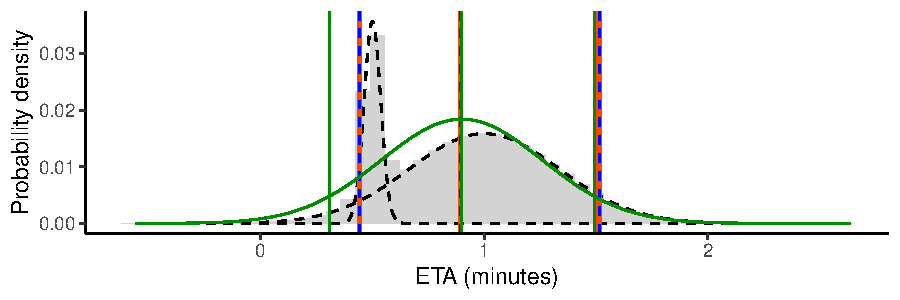
\includegraphics[width=.8\textwidth]{figure/normal_approx-1} }\newline
\subfloat[Two intermediate stops\label{fig:normal_approx2}]{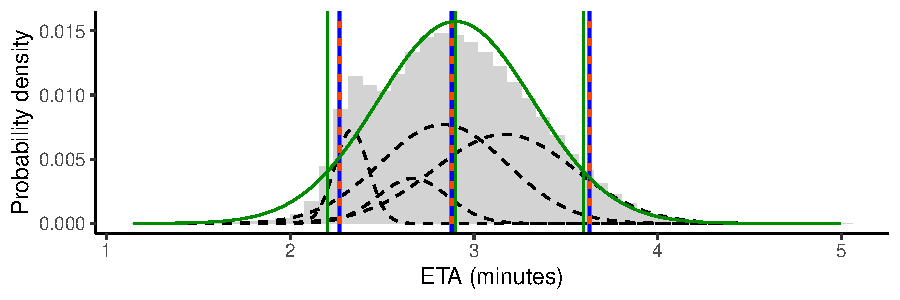
\includegraphics[width=.8\textwidth]{figure/normal_approx-2} }\newline
\subfloat[Three intermediate stops\label{fig:normal_approx3}]{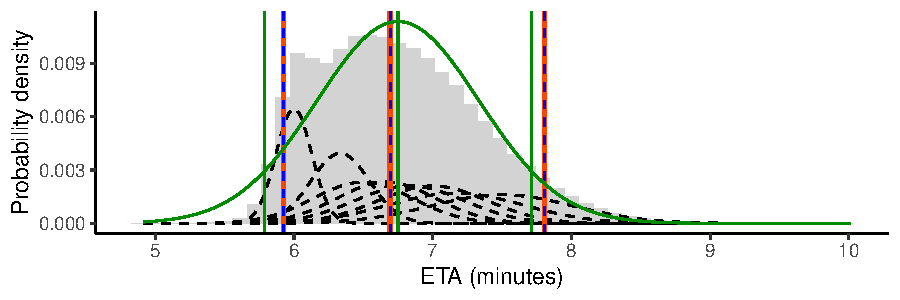
\includegraphics[width=.8\textwidth]{figure/normal_approx-3} }\newline
\subfloat[Eight intermediate stops\label{fig:normal_approx4}]{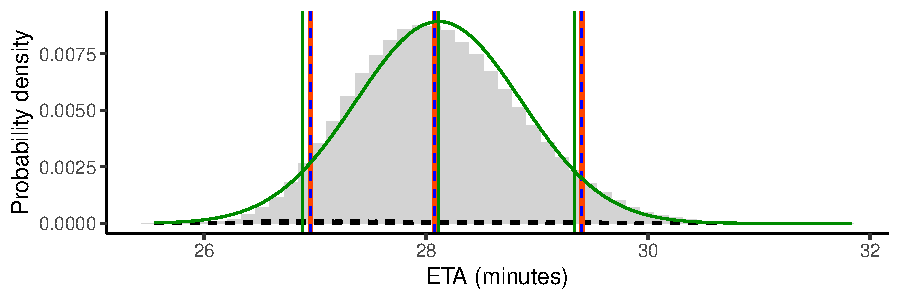
\includegraphics[width=.8\textwidth]{figure/normal_approx-4} }

}

\caption[Normal approximation for a series of stops ahead]{Normal approximation for a series of stops ahead. The true distribution is shown by the histogram with the underlying components (dashed curves). The red vertical lines represent the sample quantiles, while the dashed blue lines represent the approximated quantiles using the optimisation algorithm. Finally, the green curve and corresponding vertical lines represent the single normal approximation.}\label{fig:normal_approx}
\end{figure}


\end{knitrout}


To use a mixture of normals to incorporate stopping uncertainty, we express the mean and uncertainty as vectors $\tilde\mu$ and $\tilde\sigma^2$, respectively, along with a third vector $\tilde\pi$ denoting the $\tilde N$ mixture weights\footnote{We are using the tilde over parameters, e.g., $\tilde x$, to help distinguish them from others used throughout the thesis}, such that
\begin{equation}
\label{eq:ch5:mixture_weight_spec}
\tilde\pi_i > 0, i = 1, \ldots, \tilde N
\text{ and } \sum_{i=1}^{\tilde N} \tilde\pi_i = 1.
\end{equation}
The arrival time at stop $j + n$ is given by
\begin{equation}
\label{eq:arrival_time_normal_approx}
\Tarr_{j+n} | \tilde\mu, \tilde\sigma^2, \tilde\pi, \RouteNWstate =
\sum_{\ell=j}^{j+n-1} \RouteNWstateseg_\ell +
\sum_{i=1}^{\tilde N} \tilde\pi_i z_i,\quad
z_i \sim \Normal{\tilde\mu_i}{\tilde\sigma^2_i}.
\end{equation}


Each component $i$ has an indicator of whether or not it stopped at stop $m$, $I_{im} = \{0,1\}$, giving the total dwell time as
\begin{equation}
\label{eq:mixture_dwell_times}
\begin{split}
\tilde\mu_i &= \sum_{m=j}^{j+n} I_{im} \dwell_m \\
\tilde\sigma_i^2 &= \sum_{m=j}^{j+n} I_{im} \dwellvar_m
\end{split}
\end{equation}
which assumes dwell times at individual stops are independent of each other.

The vector of indicators is a branching tree for each stop; all current components get duplicated, and one is assigned $I_{i,m+1} = 1$ and the other 0.


Finally, mixture weights are obtained through the stopping probability at each stop, $\pi_j$:
\begin{equation}
\label{eq:ch5:mixture_weights}
\begin{split}
\tilde\pi_i &= \prod_{m=j}^{j+n} \tilde p_{im} \\
\tilde p_{im} &=
\begin{cases}
\pi_m & \text{if } I_{im} = 1 \\
1 - \pi_m & \text{otherwise.}
\end{cases}
\end{split}
\end{equation}


The mixture approximation works okay for a few stops ahead, but after some time the mixture weights become small and the components combine into more-or-less a single one, as shown in \cref{fig:normal_approx}. To prevent $\tilde N$ from becoming too large, the full distribution is simplified into a single component with mean and variance
\begin{equation}
\label{eq:mixture_mean}
\begin{split}
\E{\Tarr_m | \tilde\pi, \tilde\mu, \tilde\sigma^2, \RouteNWstate} &=
\E{\sum_{\ell=j}^{j+n-1} \RouteNWstateseg_\ell +
  \sum_{i=1}^{\tilde N} \tilde\pi_i z_i}
= \sum_{\ell=j}^{j+n-1} \E{\RouteNWstateseg_\ell} +
  \sum_{i=1}^{\tilde N} \tilde\pi_i \E{z_i} \\
&= \sum_{\ell=j}^{j+n-1} \hat\RouteNWstateseg_\ell +
  \sum_{i=1}^{\tilde N} \tilde\pi_i \tilde\mu_i
\end{split}
\end{equation}
and
\begin{equation}
\label{eq:mixture_variance}
\begin{split}
\Var{\Tarr_m | \tilde\pi, \tilde\mu, \tilde\sigma^2, \RouteNWstate} &=
\Var{\sum_{\ell=j}^{j+n-1} \RouteNWstateseg_\ell +
  \sum_{i=1}^{\tilde N} \tilde\pi_i z_i}
= \sum_{\ell=j}^{j+n-1} \Var{\RouteNWstateseg_\ell} +
  \sum_{i=1}^{\tilde N} \tilde\pi_i^2 \Var{z_i} \\
&= \sum_{\ell=j}^{j+n-1} \hat\RouteNWstatesegvar_\ell +
  \sum_{i=1}^{\tilde N} \tilde\pi_i \tilde\sigma_i^2
\end{split}
\end{equation}
respectively, assuming segment travel time and dwell time are independent---assuming otherwise makes this model impossible to work with; indeed, this model versus the particle filter (which makes no such assumption) is effectively testing the viability of this assumption.


For quantiles $q_\alpha$ we need to use an optimisation algorithm to solve
\begin{equation}
\label{eq:mixture_quadratic}
\left[
  p\left(\Tarr_m | \tilde\pi, \tilde\mu, \tilde\sigma^2, \RouteNWstate\right) - q_\alpha
\right]^2 = 0
\end{equation}
which is straightforward using Brent's Algorithm \citep{Brent_1971}, which is implemented in the Boost C++ library \citep{cn}.



However, after eight stops, the number of components is $2^8 = 256$, after which point it would be more efficient to use the particle filter. Instead, we use a simplification criteria such that, when passed, a single new component is close enough in approximation to the set of components that it can replace them. We have chosen to compare quantiles, and if the maximum absolute difference is less than one minute\footnote{When providing \glspl{eta} to commuters, they are rounded to the nearest minute, anyway.}, we replace the set of components with a single new one with mean and variance as specified in \cref{eq:mixture_mean,eq:mixture_variance}. At subsequent stops, the process repeats, and we iteratively check if a single distribution is an adequate approximation.


We also need to prevent the mixture from becoming too large: if $\tilde N > 8$, we combine components with $\tilde\pi_i < \frac{1}{2}\max_i(\pi_i)$, using appropriately modified versions of \cref{eq:mixture_mean,eq:mixture_variance}. In practice, after about five stops the distribution is approximately normal, and the error is minimal. \textcolor{red}{a figure for this}
